\PassOptionsToPackage{unicode}{hyperref}
\PassOptionsToPackage{hyphens}{url}
\PassOptionsToPackage{dvipsnames,svgnames,x11names}{xcolor}
\documentclass[
  letterpaper,
  DIV=11,
  numbers=noendperiod]{scrartcl}
\usepackage{xcolor}
\usepackage{amsmath,amssymb}
\setcounter{secnumdepth}{-\maxdimen} % remove section numbering
\usepackage{iftex}
\ifPDFTeX
  \usepackage[T1]{fontenc}
  \usepackage[utf8]{inputenc}
  \usepackage{textcomp} % provide euro and other symbols
\else % if luatex or xetex
  \usepackage{unicode-math} % this also loads fontspec
  \defaultfontfeatures{Scale=MatchLowercase}
  \defaultfontfeatures[\rmfamily]{Ligatures=TeX,Scale=1}
\fi
\usepackage{lmodern}
\ifPDFTeX\else
\fi
\IfFileExists{upquote.sty}{\usepackage{upquote}}{}
\IfFileExists{microtype.sty}{% use microtype if available
  \usepackage[]{microtype}
  \UseMicrotypeSet[protrusion]{basicmath} % disable protrusion for tt fonts
}{}
\makeatletter
\@ifundefined{KOMAClassName}{% if non-KOMA class
  \IfFileExists{parskip.sty}{%
    \usepackage{parskip}
  }{% else
    \setlength{\parindent}{0pt}
    \setlength{\parskip}{6pt plus 2pt minus 1pt}}
}{% if KOMA class
  \KOMAoptions{parskip=half}}
\makeatother
\makeatletter
\ifx\paragraph\undefined\else
  \let\oldparagraph\paragraph
  \renewcommand{\paragraph}{
    \@ifstar
      \xxxParagraphStar
      \xxxParagraphNoStar
  }
  \newcommand{\xxxParagraphStar}[1]{\oldparagraph*{#1}\mbox{}}
  \newcommand{\xxxParagraphNoStar}[1]{\oldparagraph{#1}\mbox{}}
\fi
\ifx\subparagraph\undefined\else
  \let\oldsubparagraph\subparagraph
  \renewcommand{\subparagraph}{
    \@ifstar
      \xxxSubParagraphStar
      \xxxSubParagraphNoStar
  }
  \newcommand{\xxxSubParagraphStar}[1]{\oldsubparagraph*{#1}\mbox{}}
  \newcommand{\xxxSubParagraphNoStar}[1]{\oldsubparagraph{#1}\mbox{}}
\fi
\makeatother

\usepackage{color}
\usepackage{fancyvrb}
\newcommand{\VerbBar}{|}
\newcommand{\VERB}{\Verb[commandchars=\\\{\}]}
\DefineVerbatimEnvironment{Highlighting}{Verbatim}{commandchars=\\\{\}}
\usepackage{framed}
\definecolor{shadecolor}{RGB}{241,243,245}
\newenvironment{Shaded}{\begin{snugshade}}{\end{snugshade}}
\newcommand{\AlertTok}[1]{\textcolor[rgb]{0.68,0.00,0.00}{#1}}
\newcommand{\AnnotationTok}[1]{\textcolor[rgb]{0.37,0.37,0.37}{#1}}
\newcommand{\AttributeTok}[1]{\textcolor[rgb]{0.40,0.45,0.13}{#1}}
\newcommand{\BaseNTok}[1]{\textcolor[rgb]{0.68,0.00,0.00}{#1}}
\newcommand{\BuiltInTok}[1]{\textcolor[rgb]{0.00,0.23,0.31}{#1}}
\newcommand{\CharTok}[1]{\textcolor[rgb]{0.13,0.47,0.30}{#1}}
\newcommand{\CommentTok}[1]{\textcolor[rgb]{0.37,0.37,0.37}{#1}}
\newcommand{\CommentVarTok}[1]{\textcolor[rgb]{0.37,0.37,0.37}{\textit{#1}}}
\newcommand{\ConstantTok}[1]{\textcolor[rgb]{0.56,0.35,0.01}{#1}}
\newcommand{\ControlFlowTok}[1]{\textcolor[rgb]{0.00,0.23,0.31}{\textbf{#1}}}
\newcommand{\DataTypeTok}[1]{\textcolor[rgb]{0.68,0.00,0.00}{#1}}
\newcommand{\DecValTok}[1]{\textcolor[rgb]{0.68,0.00,0.00}{#1}}
\newcommand{\DocumentationTok}[1]{\textcolor[rgb]{0.37,0.37,0.37}{\textit{#1}}}
\newcommand{\ErrorTok}[1]{\textcolor[rgb]{0.68,0.00,0.00}{#1}}
\newcommand{\ExtensionTok}[1]{\textcolor[rgb]{0.00,0.23,0.31}{#1}}
\newcommand{\FloatTok}[1]{\textcolor[rgb]{0.68,0.00,0.00}{#1}}
\newcommand{\FunctionTok}[1]{\textcolor[rgb]{0.28,0.35,0.67}{#1}}
\newcommand{\ImportTok}[1]{\textcolor[rgb]{0.00,0.46,0.62}{#1}}
\newcommand{\InformationTok}[1]{\textcolor[rgb]{0.37,0.37,0.37}{#1}}
\newcommand{\KeywordTok}[1]{\textcolor[rgb]{0.00,0.23,0.31}{\textbf{#1}}}
\newcommand{\NormalTok}[1]{\textcolor[rgb]{0.00,0.23,0.31}{#1}}
\newcommand{\OperatorTok}[1]{\textcolor[rgb]{0.37,0.37,0.37}{#1}}
\newcommand{\OtherTok}[1]{\textcolor[rgb]{0.00,0.23,0.31}{#1}}
\newcommand{\PreprocessorTok}[1]{\textcolor[rgb]{0.68,0.00,0.00}{#1}}
\newcommand{\RegionMarkerTok}[1]{\textcolor[rgb]{0.00,0.23,0.31}{#1}}
\newcommand{\SpecialCharTok}[1]{\textcolor[rgb]{0.37,0.37,0.37}{#1}}
\newcommand{\SpecialStringTok}[1]{\textcolor[rgb]{0.13,0.47,0.30}{#1}}
\newcommand{\StringTok}[1]{\textcolor[rgb]{0.13,0.47,0.30}{#1}}
\newcommand{\VariableTok}[1]{\textcolor[rgb]{0.07,0.07,0.07}{#1}}
\newcommand{\VerbatimStringTok}[1]{\textcolor[rgb]{0.13,0.47,0.30}{#1}}
\newcommand{\WarningTok}[1]{\textcolor[rgb]{0.37,0.37,0.37}{\textit{#1}}}

\usepackage{longtable,booktabs,array}
\newcounter{none} % for unnumbered tables
\usepackage{calc} % for calculating minipage widths
\usepackage{etoolbox}
\makeatletter
\patchcmd\longtable{\par}{\if@noskipsec\mbox{}\fi\par}{}{}
\makeatother
\IfFileExists{footnotehyper.sty}{\usepackage{footnotehyper}}{\usepackage{footnote}}
\makesavenoteenv{longtable}
\usepackage{graphicx}
\makeatletter
\newsavebox\pandoc@box
\newcommand*\pandocbounded[1]{% scales image to fit in text height/width
  \sbox\pandoc@box{#1}%
  \Gscale@div\@tempa{\textheight}{\dimexpr\ht\pandoc@box+\dp\pandoc@box\relax}%
  \Gscale@div\@tempb{\linewidth}{\wd\pandoc@box}%
  \ifdim\@tempb\p@<\@tempa\p@\let\@tempa\@tempb\fi% select the smaller of both
  \ifdim\@tempa\p@<\p@\scalebox{\@tempa}{\usebox\pandoc@box}%
  \else\usebox{\pandoc@box}%
  \fi%
}
\def\fps@figure{htbp}
\makeatother

\setlength{\emergencystretch}{3em} % prevent overfull lines

\providecommand{\tightlist}{%
  \setlength{\itemsep}{0pt}\setlength{\parskip}{0pt}}

\KOMAoption{captions}{tableheading}
\makeatletter
\@ifpackageloaded{caption}{}{\usepackage{caption}}
\AtBeginDocument{%
\ifdefined\contentsname
  \renewcommand*\contentsname{Table of contents}
\else
  \newcommand\contentsname{Table of contents}
\fi
\ifdefined\listfigurename
  \renewcommand*\listfigurename{List of Figures}
\else
  \newcommand\listfigurename{List of Figures}
\fi
\ifdefined\listtablename
  \renewcommand*\listtablename{List of Tables}
\else
  \newcommand\listtablename{List of Tables}
\fi
\ifdefined\figurename
  \renewcommand*\figurename{Figure}
\else
  \newcommand\figurename{Figure}
\fi
\ifdefined\tablename
  \renewcommand*\tablename{Table}
\else
  \newcommand\tablename{Table}
\fi
}
\@ifpackageloaded{float}{}{\usepackage{float}}
\floatstyle{ruled}
\@ifundefined{c@chapter}{\newfloat{codelisting}{h}{lop}}{\newfloat{codelisting}{h}{lop}[chapter]}
\floatname{codelisting}{Listing}
\newcommand*\listoflistings{\listof{codelisting}{List of Listings}}
\makeatother
\makeatletter
\makeatother
\makeatletter
\@ifpackageloaded{caption}{}{\usepackage{caption}}
\@ifpackageloaded{subcaption}{}{\usepackage{subcaption}}
\makeatother
\usepackage{bookmark}
\IfFileExists{xurl.sty}{\usepackage{xurl}}{} % add URL line breaks if available
\urlstyle{same}
\hypersetup{
  pdftitle={Python test drive},
  pdfauthor={Jun Allard},
  colorlinks=true,
  linkcolor={blue},
  filecolor={Maroon},
  citecolor={Blue},
  urlcolor={Blue},
  pdfcreator={LaTeX via pandoc}}

\ifXeTeX
\special{pdf:trailerid [ <bda0b1a278e4a81931b410346d29c04f> <bda0b1a278e4a81931b410346d29c04f> ]}
\fi
\ifPDFTeX
\pdftrailerid{}
\pdftrailer{/ID [ <bda0b1a278e4a81931b410346d29c04f> <bda0b1a278e4a81931b410346d29c04f> ]}
\fi
\ifLuaTeX
\pdfvariable trailerid {[ <bda0b1a278e4a81931b410346d29c04f> <bda0b1a278e4a81931b410346d29c04f> ]}
\fi

\title{Python test drive}
\usepackage{etoolbox}
\makeatletter
\providecommand{\subtitle}[1]{% add subtitle to \maketitle
  \apptocmd{\@title}{\par {\large #1 \par}}{}{}
}
\makeatother
\subtitle{Physics 230A/146A --- Biological Physics}
\author{Jun Allard}
\date{}
\begin{document}
\maketitle


\subsection{What this notebook is for}\label{what-this-notebook-is-for}

Scaffolding, not course material.
It exists to prove that the four things a lecture notebook needs to do all work, in all five output formats, before any real content is written into one.

Those four things are the four code chunks below.
Two of them run when the site is built, and you are reading their results.
Two of them do not, and are waiting for you to run them.

This document is also the only place in the repository where Python executes.
The problem sets are deliberately language-agnostic: where one says ``write code'', write it in whatever language you intend to use for the rest of your degree.

\subsection{A chunk that runs and produces a number}\label{a-chunk-that-runs-and-produces-a-number}

This one executes during the build.
The value below was computed on the machine that built this page, not typed in by hand.

\begin{Shaded}
\begin{Highlighting}[]
\ImportTok{import}\NormalTok{ numpy }\ImportTok{as}\NormalTok{ np}

\CommentTok{\# A number with enough decimals that it could not plausibly have been written out by hand.}
\CommentTok{\# If the build is executing code, this is the reciprocal of the golden ratio; if it is not, this cell shows as unexecuted and the claim is obviously false.}
\NormalTok{phi }\OperatorTok{=}\NormalTok{ (}\DecValTok{1} \OperatorTok{+}\NormalTok{ np.sqrt(}\DecValTok{5}\NormalTok{)) }\OperatorTok{/} \DecValTok{2}
\BuiltInTok{print}\NormalTok{(}\SpecialStringTok{f"1/phi = }\SpecialCharTok{\{}\DecValTok{1} \OperatorTok{/}\NormalTok{ phi}\SpecialCharTok{:.12f\}}\SpecialStringTok{"}\NormalTok{)}
\end{Highlighting}
\end{Shaded}

\begin{verbatim}
1/phi = 0.618033988750
\end{verbatim}

\subsection{A chunk that runs and produces a figure}\label{a-chunk-that-runs-and-produces-a-figure}

Also executed at build time.
The figure is generated, not a file committed to the repository --- which is what distinguishes a lecture notebook from a problem set, whose figures are hand-authored PDFs under version control.

\begin{Shaded}
\begin{Highlighting}[]
\ImportTok{import}\NormalTok{ matplotlib.pyplot }\ImportTok{as}\NormalTok{ plt}

\NormalTok{t }\OperatorTok{=}\NormalTok{ np.linspace(}\DecValTok{0}\NormalTok{, }\DecValTok{10}\NormalTok{, }\DecValTok{400}\NormalTok{)}

\NormalTok{fig, ax }\OperatorTok{=}\NormalTok{ plt.subplots(figsize}\OperatorTok{=}\NormalTok{(}\FloatTok{5.5}\NormalTok{, }\FloatTok{3.2}\NormalTok{))}
\ControlFlowTok{for}\NormalTok{ k }\KeywordTok{in}\NormalTok{ (}\FloatTok{1.0}\NormalTok{, }\FloatTok{0.5}\NormalTok{, }\FloatTok{0.25}\NormalTok{):}
\NormalTok{    ax.plot(t, np.exp(}\OperatorTok{{-}}\NormalTok{k }\OperatorTok{*}\NormalTok{ t), label}\OperatorTok{=}\SpecialStringTok{f"$k = }\SpecialCharTok{\{}\NormalTok{k}\SpecialCharTok{\}}\SpecialStringTok{$"}\NormalTok{)}

\NormalTok{ax.set\_xlabel(}\StringTok{"time $t$"}\NormalTok{)}
\NormalTok{ax.set\_ylabel(}\StringTok{"$e\^{}\{{-}kt\}$"}\NormalTok{)}
\NormalTok{ax.set\_xlim(}\DecValTok{0}\NormalTok{, }\DecValTok{10}\NormalTok{)}
\NormalTok{ax.set\_ylim(}\DecValTok{0}\NormalTok{, }\DecValTok{1}\NormalTok{)}
\NormalTok{ax.legend(frameon}\OperatorTok{=}\VariableTok{False}\NormalTok{)}
\NormalTok{fig.tight\_layout()}
\NormalTok{plt.show()}
\end{Highlighting}
\end{Shaded}

\begin{figure}[H]

\centering{

\pandocbounded{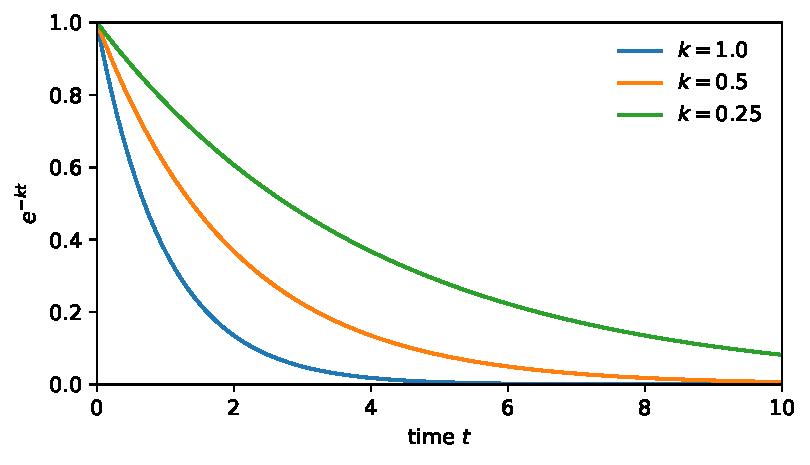
\includegraphics[keepaspectratio,alt={Three curves decaying from one towards zero over ten units of time, the steepest labelled k equals one and the shallowest k equals one quarter.}]{python-test-drive_files/figure-latex/fig-decay-output-1.pdf}}

}

\caption{\label{fig-decay}Exponential decay at three rates. Generated at build time by matplotlib.}

\end{figure}%

\subsection{A chunk that is complete, but left for you to run}\label{a-chunk-that-is-complete-but-left-for-you-to-run}

The code below is finished and correct.
It is deliberately \emph{not} executed when the site is built, so there is no output here to read --- running it is your job, and it is the simplest test of whether your setup actually works.

Open this notebook's \texttt{.ipynb} version, put your cursor in the cell, and run it.

\begin{Shaded}
\begin{Highlighting}[]
\CommentTok{\# Should print the same value as the first chunk above.}
\CommentTok{\# If it does, your environment is running the same numpy the build did.}
\ImportTok{import}\NormalTok{ numpy }\ImportTok{as}\NormalTok{ np}

\NormalTok{phi }\OperatorTok{=}\NormalTok{ (}\DecValTok{1} \OperatorTok{+}\NormalTok{ np.sqrt(}\DecValTok{5}\NormalTok{)) }\OperatorTok{/} \DecValTok{2}
\BuiltInTok{print}\NormalTok{(}\SpecialStringTok{f"1/phi = }\SpecialCharTok{\{}\DecValTok{1} \OperatorTok{/}\NormalTok{ phi}\SpecialCharTok{:.12f\}}\SpecialStringTok{"}\NormalTok{)}
\BuiltInTok{print}\NormalTok{(}\SpecialStringTok{f"numpy }\SpecialCharTok{\{}\NormalTok{np}\SpecialCharTok{.}\NormalTok{\_\_version\_\_}\SpecialCharTok{\}}\SpecialStringTok{"}\NormalTok{)}
\end{Highlighting}
\end{Shaded}

\subsection{A chunk that is yours to write}\label{a-chunk-that-is-yours-to-write}

Yours to fill in.
Plot \(\sin(t)\) against \(t\) over the same range as the figure above, using whatever you can remember or work out from the second chunk.

A chunk holding nothing but a comment is still a chunk; a chunk holding nothing at all is dropped from every output, so a stub always needs at least one line in it.

\begin{Shaded}
\begin{Highlighting}[]
\CommentTok{\# Your code here.}
\end{Highlighting}
\end{Shaded}

\subsection{What should be true}\label{what-should-be-true}

If the pipeline is working, then in the \texttt{html} and \texttt{pdf} versions of this page the first two chunks show their results and the last two show only code.
In the \texttt{.ipynb} version all four arrive as runnable code cells, and ``Run All'' completes without error.




\end{document}
